The human brain is composed of billions of neurons, interconnected electrically excitable cells that form the basis of our intelligence. Each neuron has synapses that receive electrical signals from multiple other neurons. If the sum of these inputs is greater than a certain value, the neuron fires, generating a voltage down its axon. The axon, or the output of the neuron cell, is itself connected to a synapse of another neuron. The interconnections of these neurons form a massive network, where a huge number of inputs are processed in parallel to a set of outputs. The basis of artificial neural networks is to simulate the mathematical properties of these neurons in order to perform similar tasks of mass parallel computation.


\subsection{Single Artificial Neuron}

\begin{figure}[ht]
	\centering
	\def\layersep{2.5cm}
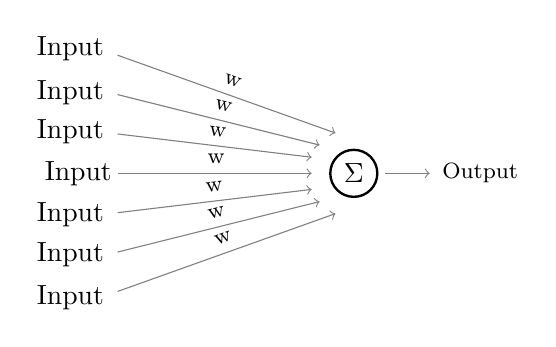
\begin{tikzpicture}[shorten >=1pt,->,draw=black!50, node distance=\layersep]
    \tikzstyle{every pin edge}=[<-,shorten <=1pt]
    \tikzstyle{neuron}=[circle,line width=0.3mm,draw=black,minimum size=17pt,inner sep=0pt]
    \tikzstyle{annot} = [text width=4em, text centered]


    \draw[->] (-3,1.5) -- (-.2,.5) node[sloped,midway,above] {\footnotesize w} node[left=3.4cm,above=.8cm]{Input};
    \draw[->] (-3,1) -- (-.4,.35) node[sloped,midway,above] {\footnotesize w} node[left=3.2cm,above=.4cm]{Input};
    \draw[->] (-3,0.5) -- (-.5,.2) node[sloped,midway,above] {\footnotesize w} node[left=3.1cm,above=.05cm]{Input};
    \draw[->] (-3,0) -- (-.5,0) node[sloped,midway,above] {\footnotesize w} node[left=2.45cm]{Input};
    \draw[->] (-3,-0.5) -- (-.5,-.2) node[sloped,midway,above] {\footnotesize w} node[left=3.1cm,below=.05cm]{Input};
    \draw[->] (-3,-1) -- (-.4,-.35) node[sloped,midway,above] {\footnotesize w} node[left=3.2cm,below=.4cm]{Input};
    \draw[->] (-3,-1.5) -- (-.2,-.5) node[sloped,midway,above] {\footnotesize w} node[left=3.4cm,below=.8cm]{Input};
    
    \node[neuron] (0,0) {$\Sigma$};

    \draw[->] (.4,0) -- (1,0) node[right] {\footnotesize Output};
\end{tikzpicture}
	\caption{Single Neuron Diagram}
\end{figure}

An artificial neuron is simply a mathematical model of a biological neuron, and therefore its functionality is very similar. Each artificial neuron has multiple inputs, each one the output of a different neuron. In addition, each neuron has a weight for each input, a bias term, an activation function, and one output. The output of one neuron becomes the input of another, connected neurons. The output of a neuron is expressed mathematically for $n$ inputs $x$ and weights $w$, a bias term $b$, and activation function $O(x)$:

\begin{align*}
	\text{activation} = \sum_{i=0}^{n}x_i w_i + b\\
	\text{output} = O(\text{activation})
	\,.
\end{align*}

A weight is a positive or negative number that governs the impact of of its respective input on the neuron's single output. The bias term is a number that is added to the summation of weights and inputs. The bias term allows us to make affine transformations on the domain of the activation function. 

In biologically inspired neurons, the activation function is a binary step function. If the activation function's input is less than a certain threshold, the output is zero. If it is greater than the threshold, the output is one. However, a binary output can be somewhat limiting for many applications of neural networks. For example, many of Fido's outputs are gradient rather than binary; as an example, Fido can set the brightness of an LED. Because of this, alternate activation functions giving gradient outputs are used. One such function is the sigmoid function, expressed as such:

\begin{equation}
	O(a) = \cfrac{1}{1+e^{-\frac{a}{p}}}
	\,,
\end{equation}

\noindent for each output $O$, activation $a$, and constant $p$. The sigmoid activation function can also be graphed as below.

\begin{figure}[ht]
	\centering
	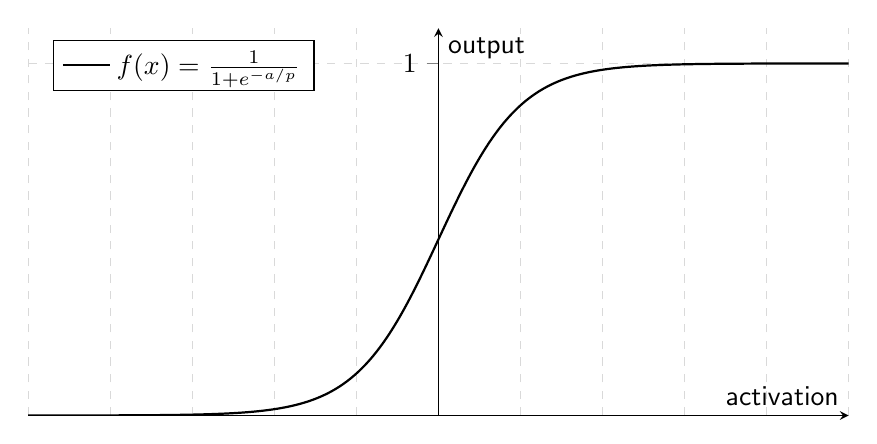
\begin{tikzpicture}[font=\sffamily]
    \begin{axis}[
    	legend pos=north west,
        axis x line=middle,
        axis y line=middle,
        grid = major,
        width=12cm,
        height=6.5cm,
        grid style={dashed, gray!30},
        xmin=-1,xmax= 1,ymin= 0,ymax= 1.1,
        xlabel=activation,ylabel=output,
        tick align=outside,
        ytick={1},
        xmajorticks=false,
        enlargelimits=false]
      \addplot[domain=-1:1,black,thick,samples=500] {1/(1+exp(-10*x))}; 
      \addlegendentry{$f(x)=\frac{1}{1+e^{-a/p}}$}
    \end{axis} 
\end{tikzpicture}
	\caption{Sigmoid Function Graph}
\end{figure}

The sigmoid function provides us with a gradient output. However, output is still limited to positive values. An alternative activation function which allows outputs ranging from -1 to +1 is the hyperbolic tangent activation function.

\begin{figure}[ht]
	\centering
	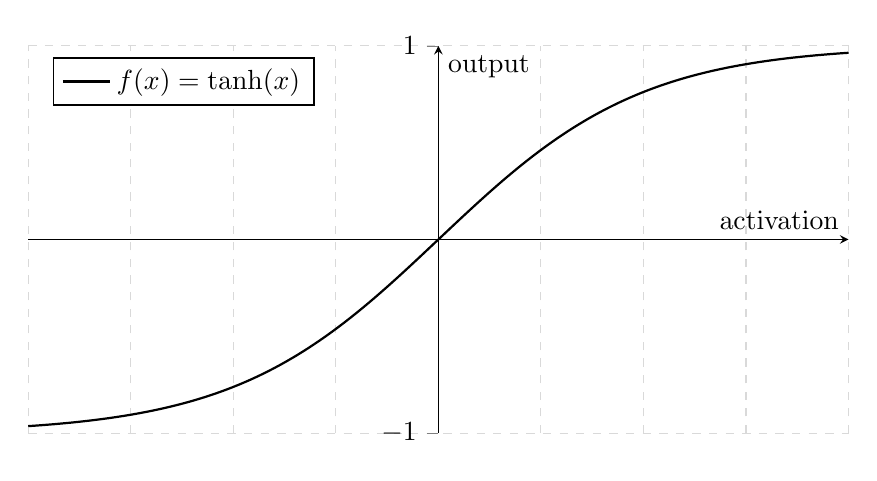
\begin{tikzpicture}
    \begin{axis}[
    	legend pos=north west,
        axis x line=middle,
        axis y line=middle,
        grid = major,
        width=12cm,
        height=6.5cm,
        grid style={dashed, gray!30},
        xmin=-2,xmax= 2,ymin= -1,ymax= 1,
        xlabel=activation,ylabel=output,
        tick align=outside,
        ytick={-1,1},
        xmajorticks=false,
        enlargelimits=false]
      \addplot[domain=-2:2,black,thick,samples=500] {tanh(x)}; 
      \addlegendentry{$f(x)=\tanh(x)$}
    \end{axis} 
\end{tikzpicture}
	\caption{Hyperbolic Tangent Function Graph}
\end{figure}

\subsection{Feed-forward Neural Network}

A traditional method of arranging artificial neurons in a neural network is called a feed-forward network. Neurons are connected as previously described: the output of each neuron is connected to one of the inputs of another neuron. These neurons are organized into layers, as described in the following figure:

\begin{figure}[ht]
	\centering
	\def\layersep{2.5cm}
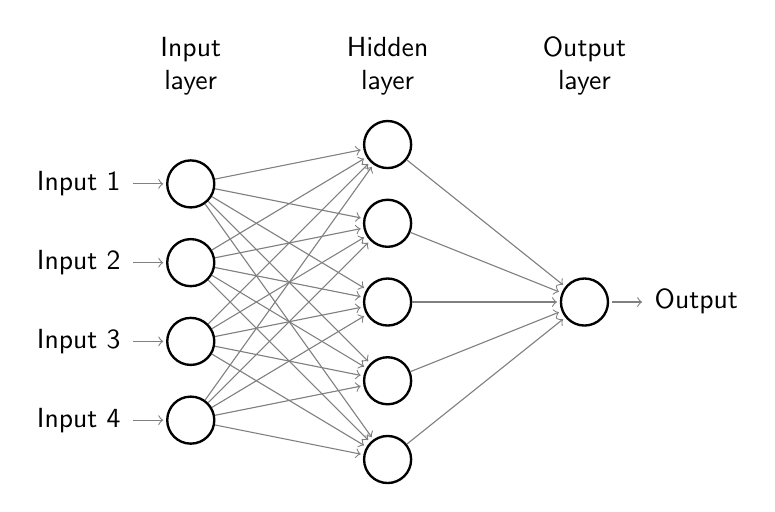
\begin{tikzpicture}[shorten >=1pt,->,draw=black!50, node distance=\layersep,font=\sffamily]
    \tikzstyle{every pin edge}=[<-,shorten <=1pt]
    \tikzstyle{neuron}=[circle,line width=0.3mm,draw=black,minimum size=17pt,inner sep=0pt]
    \tikzstyle{annot} = [text width=4em, text centered]

    \foreach \name / \y in {1,...,4}
        \node[neuron, pin=left:Input \y] (I-\name) at (0,-\y) {};

    \foreach \name / \y in {1,...,5}
        \path[yshift=0.5cm]
            node[neuron] (H-\name) at (\layersep,-\y cm) {};

    \node[neuron,pin={[pin edge={->}]right:Output}, right of=H-3] (O) {};

    \foreach \source in {1,...,4}
        \foreach \dest in {1,...,5}
            \path (I-\source) edge (H-\dest);

    \foreach \source in {1,...,5}
        \path (H-\source) edge (O);

    %\draw[->] (5,-2.9) -- (5,-5) -- (1,-5) -- (1,-4.5);
    %\node (1,-4.5) {Error back propagation}

    \node[annot,above of=H-1, node distance=1cm] (hl) {Hidden layer};
    \node[annot,left of=hl] {Input layer};
    \node[annot,right of=hl] {Output layer};
\end{tikzpicture}
	\caption{Single Output Feed-forward Network}
\end{figure}

The output of each neuron in a layer becomes an input of every neuron in the next layer. In this way, the original inputs of the neural network are ``fed forward'' layer by layer, starting from the first layer (the input layer), passing through any number of hidden layers, ending with the last layer (the output layer). The outputs of the neurons of the output layer are the outputs of the whole network.

A concrete example of a feed-forward network is that of Fido. Sensor inputs such as light and sound are sent into the input layer. The outputs of the output layer's neurons are used to change the speed of Fido's motors, the color of Fido's LEDs, and the sounds of Fido's buzzers.

\subsection{Back Propagation}

Supervised learning is a type of neural network training that modifies neuron input weights in order to reach a specific output from a specific set of inputs.  Initially the neuron weights are randomly generated, but over time the weights are adjusted to converge on the correct output.  One such method of adjusting neural weights is called back propagation \cite{werbos}.

\begin{figure}[ht]
	\centering
	\def\layersep{2.5cm}
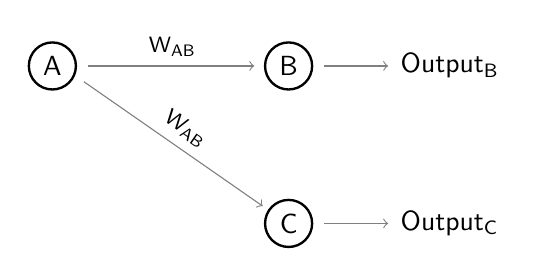
\begin{tikzpicture}[font=\sffamily,shorten >=1pt,->,draw=black!50, node distance=\layersep]
    \tikzstyle{every pin edge}=[<-,shorten <=1pt]
    \tikzstyle{neuron}=[circle,line width=0.3mm,draw=black,minimum size=17pt,inner sep=0pt]
    \tikzstyle{annot} = [text width=4em, text centered]

    \draw[->] (.45,0) -- (2.6,0) node[sloped,midway,above] {\footnotesize W\textsubscript{AB}};
    \draw[->] (.4,-.2) -- (2.7,-1.8) node[sloped,midway,above] {\footnotesize W\textsubscript{AB}};

    \draw[->] (3.45,0) -- (4.3,0) node[right=0cm]{Output\textsubscript{B}};
    \draw[->] (3.45,-2) -- (4.3,-2) node[right=0cm]{Output\textsubscript{C}};
    
    \node[neuron] at (0,0) {A};
    \node[neuron] at (3,0) {B};
    \node[neuron] at (3,-2) {C};
\end{tikzpicture}
	\caption{Single Branch in a Back Propagation Neural Network}
	\label{fig:backprop}
\end{figure}

In the most abstract sense, back propagation neural networks learn through example.  Example inputs (known as training sets) are linked to a particular target output, forming a training pair.  The first step of training is to pass in an arbitrary training set to a neural network with randomly generated weights.  The error of the network for a certain connection $\delta$ is defined as the difference between the actual output and the target output for that training set. As an example we will use the single connection described in figure \ref{fig:backprop}.  We first determine the neuron $B$ error $\delta_B$ as $\text{Target}_B - \text{Output}_B$.   Next we modify weight $W_{AB}$ as follows, defining $W_{AB}^{+}$ as the newly trained weight:

\begin{equation}
	W_{AB}^{+} = W_{AB} + (\delta_B \text{Output}_A)\,.
\end{equation}

The same approach could be taken for neuron $C$.  However, this method cannot calculate an improved weight for hidden layer neurons such as neuron $A$, as there is no predefined target.  Therefore we must calculate the error of $A$ indirectly by back propagating from the two output layer neurons, for which the error is already known.

\begin{equation}
	\delta_A = W_{AB}\text{Error}_B + W_{AC}\text{Error}_C
\end{equation}

Once the error for neuron $A$ is obtained, its trained weights can be calculated in the same fashion as done for neuron $B$.  This pattern can be repeated throughout a larger neural network in order to converge upon the target output.
